\documentclass[letterpaper,serif,tightsqueeze]{rpg_module}

\usepackage{parskip}                                                            % Add spacing between paras instead of indents
\usepackage{enumitem}                                                           % Control spacing in description list

\renewcommand{\newmonsterfont}{\bfseries}                                       % Redefine new monster headings to use a smaller font
\renewcommand{\newmonsterbottomskip}{0ex}                                       % Reduce the space below New Monster sections

\setcounter{page}{44}                                                           % Page and section numbers
\setcounter{part}{6}

\RequirePackage{fancyhdr}                                                       % Change page numbering style
\fancypagestyle{plain}{%
   \fancyhf{} % clear all header and footer fields
   \fancyfoot[C]{B\thepage} % page numbering
   \renewcommand{\headrulewidth}{0pt}
   \renewcommand{\footrulewidth}{0pt}
}
\pagestyle{plain}

% Redefine troglodyte/zombie so damage fits on one line

\monster{troglodyte}{Troglodyte}{||5|2*|120'|40'||||3|2 claws\?1 bite|1d4\x 3|1d4 each|Fighter: 2|9|Chaotic|1--8|5--40|A|25}
\monster{zombie}{Zombie}{||8|2|120'|40'||||1|1 weapon|1d8|1d8~or~weapon|Fighter: 1|12|Chaotic|2--8|4--24|Nil|20}

% Redefine veteran to be more generic for New Monster block

\monster{veteran}{Veteran}{||2|1--3|60'|20'||||1|1 weapon|1d8|1d8~or~weapon|Fighter: 1--3|9 (varies)|Any|2--8|2--12|V|10}

% 3/4 symbol

\newcommand{\threequarters}{{\usefont{T1}{lmr}{m}{n}\sfrac{3}{4}} }



\begin{document}

\onecolumn

\begin{center}
Page intentionally left blank
\end{center}

\twocolumn

\begin{newmonster}{troglodyte}
A troglodyte is an intelligent human-like reptile with a short tail,
long legs, and a spiny ``comb'' on its head and arms. Troglodytes
walk upright and use their hands as well as humans. They hate
most other creatures, and will try to kill anyone they meet. They
have a chameleon-like ability to change colors, and use it to hide
by rock walls, surprising on a roll of 1--4 (on 1d6). They secrete an
oil which produces a stench that will nauseate humans and demihumans
unless the victims save vs. Poison. Nauseated characters
will have a penalty of \minus 2 on their ``to hit'' rolls while in hand-to-hand
combat with the troglodytes.

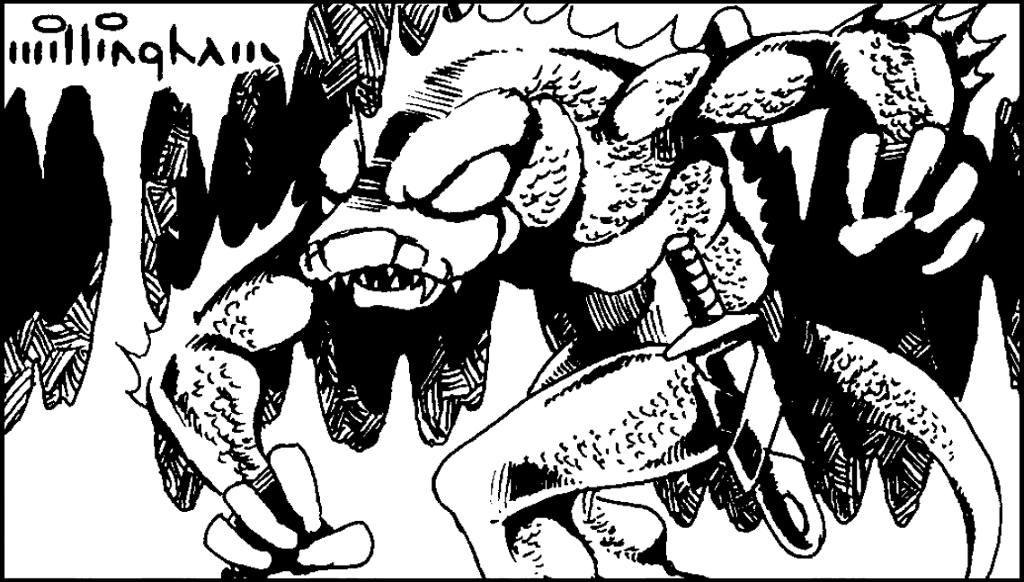
\includegraphics[width=\linewidth]{troglodyte.png}
\end{newmonster}
\vspace{-3ex}\textbf{Undead:} (see \textbf{Ghoul}, \textbf{Skeleton}, \textbf{Wight} and \textbf{Zombie})

Undead are evil creatures who have been created through dark
magic. They are unaffected by things that affect living creatures,
such as poison, and are not affected by spells which affect the
mind, such as \textbf{sleep} and \textbf{charm person}. They do not make noise.

\begin{newmonster}{veteran}
Veterans are low-level fighters, usually returning from or going to a
war. To determine each veteran's level and alignment, use the
method outlined under \textbf{Creating an NPC Party} (page B52). A
party of veterans may be of mixed levels and alignments, or the
DM may wish to give all members the same levels.
\end{newmonster}
\textbf{Were-creature} (werebear, wearboar, wererat, weretiger, or werewolf); see \textbf{Lycanthropes}.\\[1ex]
\begin{newmonster}{wight}
A wight is an \textbf{undead} spirit living in the body of a dead human or
demi-human. It can only be hit by silvered or magical weapons.
Wights are greatly feared, as they drain life energy when striking a
victim. Each hit drains one level of experience or hit die (life
energy, see page B29). EXAMPLE: A 3rd level fighter struck by a
wight becomes a 2nd level fighter, keeping only enough experience
points to be at the midpoint of 2nd level, and losing 1 hit die
of hit points. Any person totally drained of life energy by a wight
will become a wight in 1--4 days, and will be under control of the
wight who drained him or her.
\end{newmonster}
\begin{newmonster2}{wolf}{dire_wolf}
\textbf{Wolves:} Wolves are meat-eaters and hunt in packs. Though
wolves prefer the wilderness, they will occasionally be found in
caves. Captured wolf cubs can be trained like dogs (if the DM permits),
but it is difficult. If 3 wolves or less are encountered, or if a
pack is reduced to less than 50\% of its original numbers, their
morale score is 6 rather than 8.

\textbf{Dire Wolves:} Dire wolves may be found in caves, woods, or
mountains. They are larger and more ferocious than normal
wolves, and are semi-intelligent. They are fierce enemies and
usually hunt in packs. They are sometimes trained by goblins to be
used as mounts. Captured dire wolf cubs can be trained like dogs
(if the DM permits), but they are even more savage than normal
wolves.
\end{newmonster2}
\begin{newmonster}{yellow_mold}
This deadly fungus covers an area of 10 square feet (2' by 5', for
example), though many are sometimes found together. Yellow
mold can only be killed by fire; a torch will do 1--4 points of damage
to it each round. It will eat through wood and leather but does not
harm metal or stone. It does not actually attack, but if it is touched
(by a torch, for. example) the touch may cause the mold to squirt
out a 10'\x 10'\x 10' cloud of spores. There is a 50\% chance per hit
that the mold will squirt out this cloud. Anyone caught within the
cloud must save vs. Death Ray or choke to death within 6 rounds.
\end{newmonster}
\begin{newmonster}{zombie}
Zombies are undead humans or demi-humans animated by some
evil cleric or magic-user. As all undead, they may be ``Turned'' by
a cleric but are not affected by sleep or charm spells or any form
of mind reading. They are often placed to guard treasures, since
they make no noise until they attack. Zombies will always attack on
sight, but can be destroyed by normal weapons. They are slow
fighters, and always strike last (no initiative roll needed).
\end{newmonster}

\begin{onecolumnfloat}[t]
\part{Treasure}
\end{onecolumnfloat}
\begin{onecolumnfloat}[hb!]
\begin{center}
\textbf{TREASURE TYPES}
\end{center}
\vspace{1ex}
\addtolength{\tabcolsep}{0.6mm}
\begin{tabularx}{\linewidth}{clllll>{\raggedright\arraybackslash\hsize=1.9cm}X>{\raggedright\arraybackslash\hsize=4.5cm}X}
% Need a bit of a hack to get table headers spanning 2 rows unfortunately
& \multicolumn{1}{b}{1000's of} & \multicolumn{1}{b}{1000's of} & \multicolumn{1}{b}{1000's of} &
  \multicolumn{1}{b}{1000's of} & \multicolumn{1}{b}{1000's of} & \multicolumn{1}{b}{*Gems and}\\[-0.7ex]
\tableheader[b]{Type & Copper & Silver & Electrum & Gold & Platinum & Jewelry & Magic Items}
A & 25\% 1--6  & 30\% 1--6   & 20\% 1--4   & 35\% 2--12  & 25\% 1--2  & 50\% 6--36               & 30\% Any 3\\
B & 50\% 1--8  & 25\% 1--6   & 25\% 1--4   & 25\% 1--3   & Nil        & 25\% 1--6                & 10\% 1 sword, armor, or weapon\\
C & 20\% 1--12 & 30\% 1--4   & 10\% 1--4   & Nil         & Nil        & 25\% 1--4                & 10\% Any 2\\
D & 10\% 1--8  & 15\% 1--12  & Nil         & 60\% 1--6   & Nil        & 30\% 1--8                & 15\% Any 2 + 1 potion\\
E & 5\% 1--10  & 30\% 1--12  & 25\% 1--4   & 25\% 1--8   & Nil        & 10\% 1--10               & 25\% Any 3 + 1 scroll\\
F & Nil        & 10\% 2--20  & 20\% 1--8   & 45\% 1--12  & 30\% 1--3  & 20\% 2--24\?10\%~1--12   & 30\% Any 3 except weapons + 1 potion + 1 scroll\\
G & Nil        & Nil         & Nil         & 50\% 10--40 & 50\% 1--6  & 25\% 3--18\?25\%~1--10   & 35\% Any 4 + 1 scroll\\
H & 25\% 3--24 & 50\% 1--100 & 50\% 10--40 & 50\% 10--60 & 25\% 5--20 & 50\% 1--100\?50\%~10--40 & 15\% Any 4 + 1 potion + 1 scroll\\
I & Nil        & Nil         & Nil         & Nil         & 30\% 1--8  & 50\% 2--12               & 15\% Any 1\\
J & 25\% 1--4  & 10\% 1--3   & Nil         & Nil         & Nil        & Nil                      & Nil\\
K & Nil        & 30\% 1--6   & 10\% 1--2   & Nil         & Nil        & Nil                      & Nil\\
L & Nil        & Nil         & Nil         & Nil         & Nil        & 50\% 1--4\?Nil           & Nil\\
M & Nil        & Nil         & Nil         & 40\% 2--8   & 50\% 5--30 & 55\% 5--20\?45\%~2--12   & Nil\\
N & Nil        & Nil         & Nil         & Nil         & Nil        & Nil                      & 40\% 2--8 potions\\
O & Nil        & Nil         & Nil         & Nil         & Nil        & Nil                      & 50\% 1--4 scrolls\\
\end{tabularx}
% Can't have a footnote inside a float, here is a workaround
\begin{enumerate}[leftmargin=5cm,rightmargin=5cm]
\item[*] Roll twice, once for each category (Gems and Jewelry). The chances are the same unless two notations are made, in which case the order given is for ``Gems/Jewelry''.
\end{enumerate}
\end{onecolumnfloat}

The coins, gems, jewelry and magic items that a party finds during
an adventure is known as \textbf{treasure}. Wealth (coins, gems, jewelry
and other items of value) is worth experience points to the player
and allows the player to pay for better equipment, hire more retainers,
and purchase special services (from higher level spell
casters, for example). Magic items will usually give a character
abilities not normally possessed and are useful on later adventures.
Treasure is normally found in the lairs of monsters, but may be
paid to a character by a high level NPC for performing a mission or
job. Treasures are determined randomly or chosen by the DM. The
DM should always determine the contents of a large treasure
hoard before play in order to determine how best to hide and protect
the treasure from theft, and if magic items are present, the DM
may want to allow the monsters to use the items, such as a bugbear
using a \textbf{sword\+1}.

RANDOM TREASURES: To determine a monster's treasure at
random, the DM uses the following step-by-step procedure:
%\begin{description}[labelindent=1em,leftmargin=1em]
\begin{enumerate}
\item Find the Treasure Type in the monster description. Find the
same letter on the Treasure Types table hereafter; that
line will be used to find the actual treasure.
\item Read across the Treasure Type line to find which types of
treasure may be present. Each type will have a percentage
and a range. If the DM rolls (on d\%) a number equal to or
less than the percentage given, that type of treasure is
present. The DM should roll for each percentage and
make a note of what types are present.
\item Roll dice (the type depends on the range given) to find the
amount of each type of treasure (found in step 2, above) which is present.
\item If any magic items are present, the magic item subtables (page B46)
must be used to find the actual types.
\end{enumerate}

PLACED TREASURES: The DM may choose treasures instead of
rolling for them randomly, or may choose a result if rolls give too
much or too little treasure. The choices should be made carefully,
since most of the experience the characters will get will be from
treasure (usually \threequarters or more). It will often be easier for the DM to
decide how much experience to give out (considering the size and
levels of experience in the party) and place the treasures to give
this result. However, the monsters should be tough enough to
make sure that the characters earn their treasure!

ADJUSTMENTS TO TREASURE: Treasures A through O are
large, and generally only for use when large numbers or fairly difficult
monsters are encountered. The lairs of most human-like
monsters contain at least the number of creatures given as the
wilderness ``No. Appearing'' (the number in parentheses). An encounter
with less than a full lair should yield less treasure. On the
other hand if 1--4 is the ``No. Appearing'', even one will have the
normal amount of treasure, and no adjustment is necessary.

The DM may create Treasure Types other than the ones listed.
Some other valuable items could be rugs, wall hangings, rare
wines, silverware and other kitchen items, or even animal skins.
The DM should give each special item a value, in gold pieces (and,
if the optional encumbrance rules are used, an encumbrance).

To aid the DM, the average values (in gold pieces) of each treasure
type are given below. These averages do not include the possible
magic in the treasures. After rolling for treasures, the DM may refer
to this list to see whether the treasure is larger or smaller than
average and may then adjust the treasure as desired.

\begin{tabular}{>{\hfill}p{1cm} r >{\hfill}p{1cm} r >{\hfill}p{1cm} r}
A & 17,000 & F &  5,000 & J &     25\\
B &  2,000 & G & 25,000 & K &    125\\
C &  1,000 & H & 50,000 & L &    250\\
D &  4,000 & I &  8,000 & M & 15,000\\
E &  2,500\\
\end{tabular}

\end{document}
